\subsection{Evaluating Limits}\label{subsec:evaluating-limits}

\begin{enumerate}
    \item To simply evaluate $\lim_{x\to{c}}f(x)$, 
    plug in $c$ such that $f(c)=L$, the value of the limit.

    \item If $f(c)=\frac{0}{0}$, factor numerator and denominator, then cancel terms.
    
    \[lim_{x\to{0}}\frac{x^4+x^2}{x^3+3x^2}=
        \lim_{x\to{0}}\frac{x^2+1}{x+3}=\frac{1}{3}\]

    \item If $f(c)=\frac{0}{0}$ and radicals are involved, 
    then rationalize using conjugate and resubstitute.
                  
    \[lim_{x\to{9}}\frac{\sqrt{x}-3}{x-9}\]

    \item For limits that approach $\pm{\infty}$, cancel everything but 
    greatest degree terms from numerator and denominator, then re-evaluate.
\end{enumerate}

Given the problem to find the value of constant $c$ as below, observe that
when the limit is indeterminate, it is in the form $\frac{0}{0}$.
This is because a limit with just denominator as $0$ does not exist, so 
the indeterminate form is required.

\begin{gather*}
    \lim_{x\to{2}}\frac{x^2+cx+c-10}{x^2-3x+2}\\
    x^2-3x+2\vert_{x=2}=0\Rightarrow \lim_{x\to{2}}\frac{x^2+cx+c-10}{x^2-3x+2}=\frac{0}{0}\\
    x^2+cx+c-10\vert_2=3c-6=0\\
    c=2\\
\end{gather*}

\subsection{Horizontal Asymptotes}\label{subsec:horizontal-asymptotes}

Take limit to $\pm \infty$ (end behavior).

\subsection{Squeeze Theorem}\label{subsec:squeeze-theorem}

Near $x=c$, let $g(x)\leq{f(x)}\leq{h(x)}\;\forall{x}$, if $\lim_{x\to{c}}g(x)=L$ and $\lim_{x\to{c}}h(x)=L$,
then $\lim_{x\to{c}}f(x)=L$ must be true.

\bigskip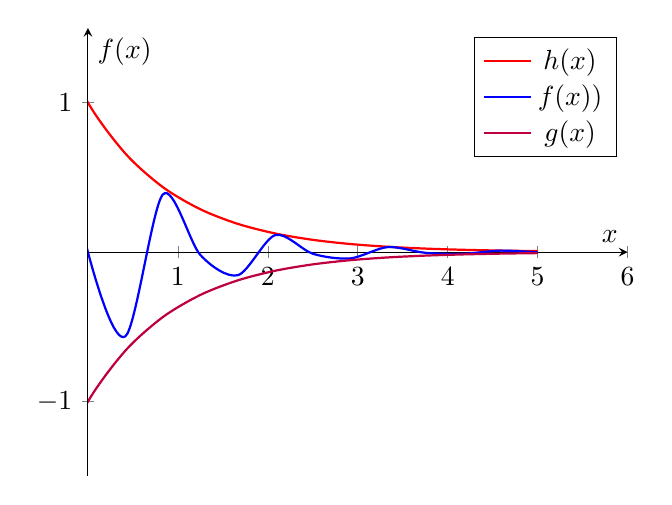
\begin{tikzpicture}
    \begin{axis}[
        xmin=0,xmax=6,
        ymin=-1.5,ymax=1.5,
        axis x line=middle,
        axis y line=middle,
        xlabel={$x$},
        ylabel={$f(x)$}
        ]
    \addplot[red,thick,smooth] {e^(-x)};
    \addlegendentry{$h(x)$}
    \addplot[blue,thick,smooth] {e^(-x)*sin(10*deg(x))};
    \addlegendentry{$f(x))$}
    \addplot[purple,thick,smooth] {-e^(-x)};
    \addlegendentry{$g(x)$}
    \end{axis}
\end{tikzpicture}

\subsection{Graphical Limits}\label{subsec:graphical-limits}

\begin{tikzpicture}
    \begin{axis}[
        xmin=-2,xmax=2,
        ymin=-2,ymax=3,
        axis x line=middle,
        axis y line=middle,
        axis line style=<->,
        xlabel={$x$},
        ylabel={$y$}
        ]
    \addplot[red,thick,domain=-1.5:1.5,<->] {x};
    \addplot[mark=*,fill=white] coordinates {(1,1)};
    \draw [dashed] (1,1) -- (1,0);
    \addlegendentry{$y=f(x)$}
    \end{axis}
\end{tikzpicture}\bigskip

Notice that the limit of $f(x)$ exists at $x=1$ though it is undefined at $(1,1)$.\\
Formally, $\lim_{x\to{1}}f(x)=1$ where $\lim_{x\to{1^-}}f(x)=\lim_{x\to{1^+}}f(x)$.

\subsection{Continuity}\label{subsec:continuity}

A function is continuous at an interior point if 
$\lim_{x\to{c}}f(x)=f(c)$.
It is continuous at a left endpoint if
$\lim_{x\to{a^+}}f(x)=f(a)$ and at a right endpoint if $\lim_{x\to{b^-}}f(x)=f(b)$.
